%!TEX root = ../template.tex
%%%%%%%%%%%%%%%%%%%%%%%%%%%%%%%%%%%%%%%%%%%%%%%%%%%%%%%%%%%%%%%%%%%%
%% chapter4.tex
%% NOVA thesis document file
%%
%% Chapter with lots of dummy text
%%%%%%%%%%%%%%%%%%%%%%%%%%%%%%%%%%%%%%%%%%%%%%%%%%%%%%%%%%%%%%%%%%%%

\typeout{NT FILE chapter4.tex}%

\chapter{Work Plan}
\label{cha:work_plan}

Figure presents a Gantt chart to illustrate an outline of the timeline and key
milestones from this point foward. The chart is divided into several phases,
each with specific tasks and deadlines.

\begin{figure}[htbp]
  \centering
  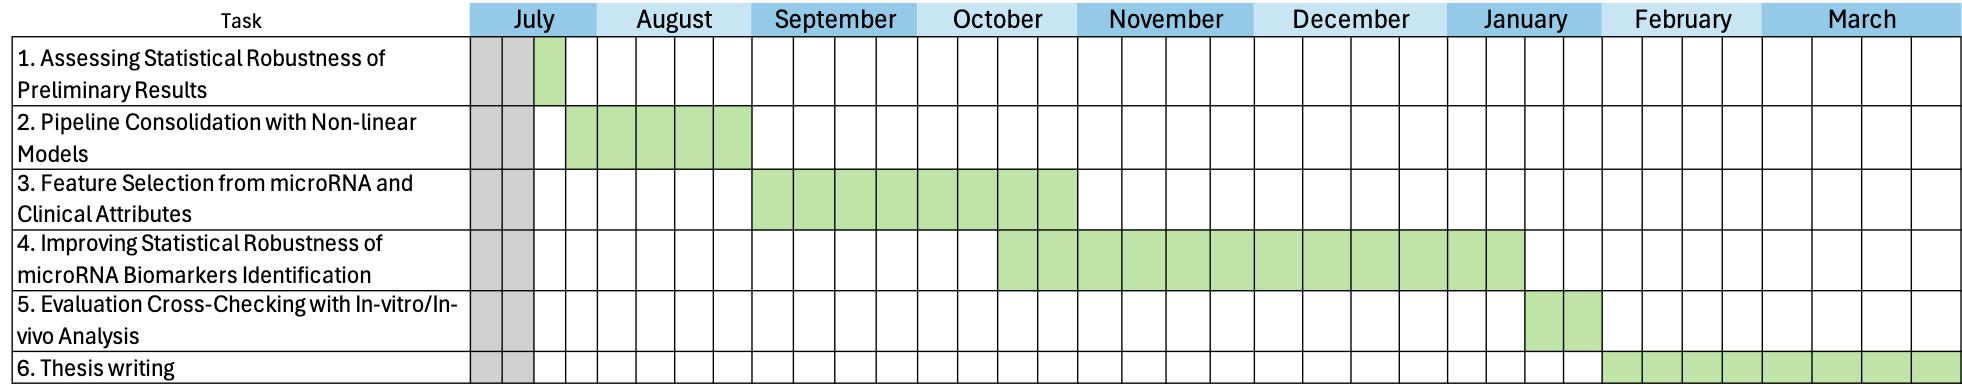
\includegraphics[width=1.0\textwidth]{/Users/JoseRomano/Documents/Tese/bca-thesis/Chapters/Figures/workplan.png}
  \caption{Gantt chart illustrating the work plan and expected timeline for the project.}
  \label{fig:gantt_chart}
\end{figure}

Although the Gantt chart provides a visual overview of the timeline, some
details may not be fully legible. For clarity, the main tasks and milestones
are listed below.

\begin{enumerate}
  \item Assessing Statistical Robustness of Preliminary Results
  \item Pipeline Consolidation with Non-linear Models
  \item Feature Selection from microRNA and Clinical Attributes
  \item Improving Statistical Robustness of microRNA Biomarkers Identification
  \item Evaluation Cross-Checking with In-vitro/In-vivo Analysis
  \item Thesis writing
\end{enumerate}